% =====================================================================
\chapter{La planta}\label{cap:planta}

\section{Qué es y qué hace}
El XK-JS1-1 es un brazo didáctico de \textbf{4 grados de libertad} que toma piezas pequeñas y las traslada. Tres movimientos son continuos y accionados por motores paso a paso; el cuarto es la garra, de dos estados.

\begin{figure}[H]
\centering
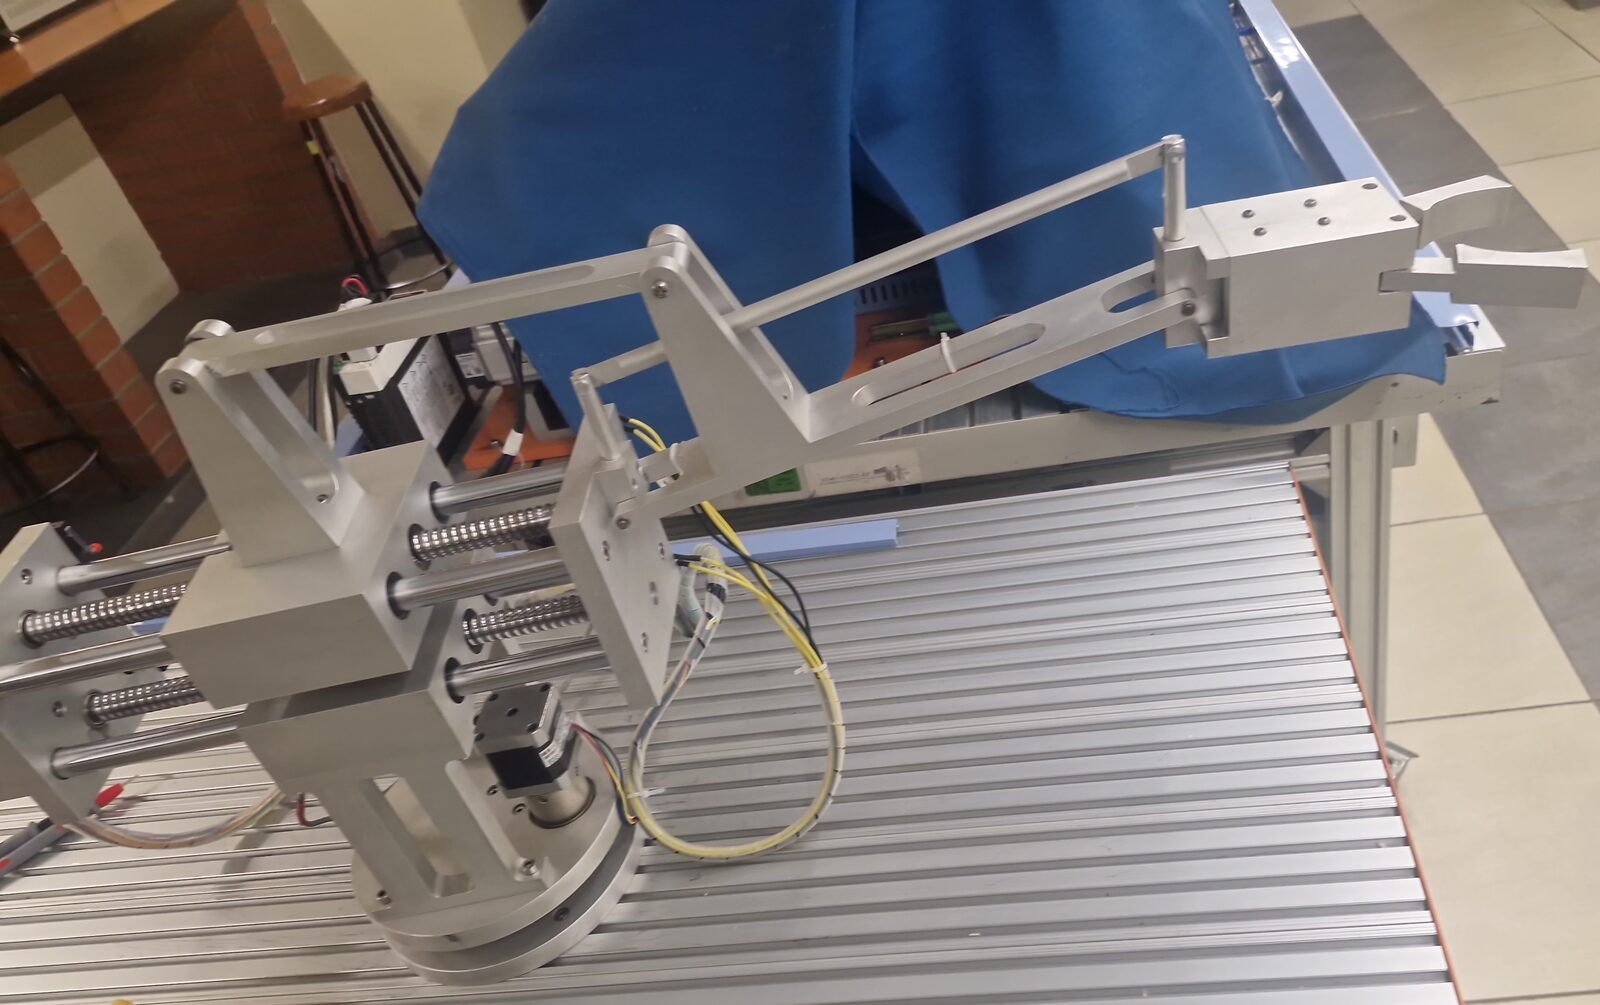
\includegraphics[width=0.62\linewidth]{brazo_vista_general.jpg}
\caption{El brazo XK-JS1-1 en el laboratorio.}
\end{figure}

\begin{center}\small
\begin{tabularx}{\linewidth}{>{\raggedright}p{2.5cm} >{\raggedright}X >{\raggedright\arraybackslash}p{4.8cm}}
\toprule
\textbf{Grado de libertad} & \textbf{Movimiento} & \textbf{Accionamiento}\\
\midrule
Base ($\theta$, motor Z) & giro alrededor del eje vertical & NEMA 17 + driver 2M530 + engranaje\\
Carro X ($s_X$) & desplaza todo el brazo: cambia el alcance & NEMA 23 + driver 2M542 + husillo inferior\\
Carro Y ($s_Y$) & mueve un bloque que, por una biela, levanta el brazo: cambia la altura & NEMA 23 + driver 2M542 + husillo superior\\
Garra & abre o cierra las mordazas & solenoide de 24~V por el relé K3 (salida Q0.7)\\
\bottomrule
\end{tabularx}
\end{center}

\section{Ficha técnica del hardware}
Datos de la auditoría del informe 1, de las hojas de datos de \codigo{global/datasheets/} y de las verificaciones hechas en la planta en octubre de 2026.

\begin{center}\small
\begin{longtable}{>{\raggedright}p{3.2cm} >{\raggedright}p{4cm} >{\raggedright\arraybackslash}p{7.8cm}}
\toprule
\textbf{Componente} & \textbf{Modelo} & \textbf{Datos clave}\\
\midrule
\endhead
PLC & Siemens S7-200 CPU 224 CN (6ES7 214-1AD23) & 14 entradas y 10 salidas digitales de 24~V DC (transistor); 2 salidas de pulsos rápidas (Q0.0, Q0.1) hasta 20~kHz; un puerto RS-485 (puerto 0) con protocolo PPI\\
Drivers X e Y & JMC 2M542-N (compatible DM542) & 20--50~V DC, 1,0--4,2~A pico; entradas PUL, DIR y ENA optoacopladas; micropasos por interruptores DIP\\
Driver base & JMC 2M530 & 18--50~V DC, 0,5--3,0~A (informe 1); tabla DIP por confirmar en su placa\\
Motores X e Y & NEMA 23, 57J1854-828 & 1,8° por paso (200 pasos/vuelta), 2,8~A por fase\\
Motor base & NEMA 17, 42J1848-604 & 1,8° por paso, 1,2~A por fase\\
Husillos X e Y & de bolas, tipo SFU1605 (SUPUESTO) & paso 5~mm/vuelta (SUPUESTO)\\
Relés K1, K2, K3 & Omron MY2N-J (24~V DC) & 2 contactos conmutados (DPDT), 5~A; K1 y K2 reparten el tren de pulsos, K3 acciona el solenoide\\
Finales de carrera X e Y & microinterruptores (informe 1: M102-011; hoja de datos: V-156-1C25) & 4 unidades, contacto NA/NC\\
Sensor de la base & LJ12A3-4-Z/BX & inductivo NPN normalmente abierto, 6--36~V DC, alcance 4~mm, 100~Hz\\
Garra & solenoide de 24~V DC & todo o nada; Q0.7 = 1 cerrada\\
Fuente & conmutada 24~V / 5~V DC & alimenta PLC, sensores y la lógica de los drivers\\
Protección & disyuntor diferencial DZ47LE-63 & 16~A, 30~mA, curva C\\
Panel & botonera & pulsadores Start, Stop, Reset, S1--S7 y selector Manual/Automático\\
\bottomrule
\end{longtable}
\end{center}

\begin{figure}[H]
\centering
\begin{minipage}[t]{0.32\linewidth}\centering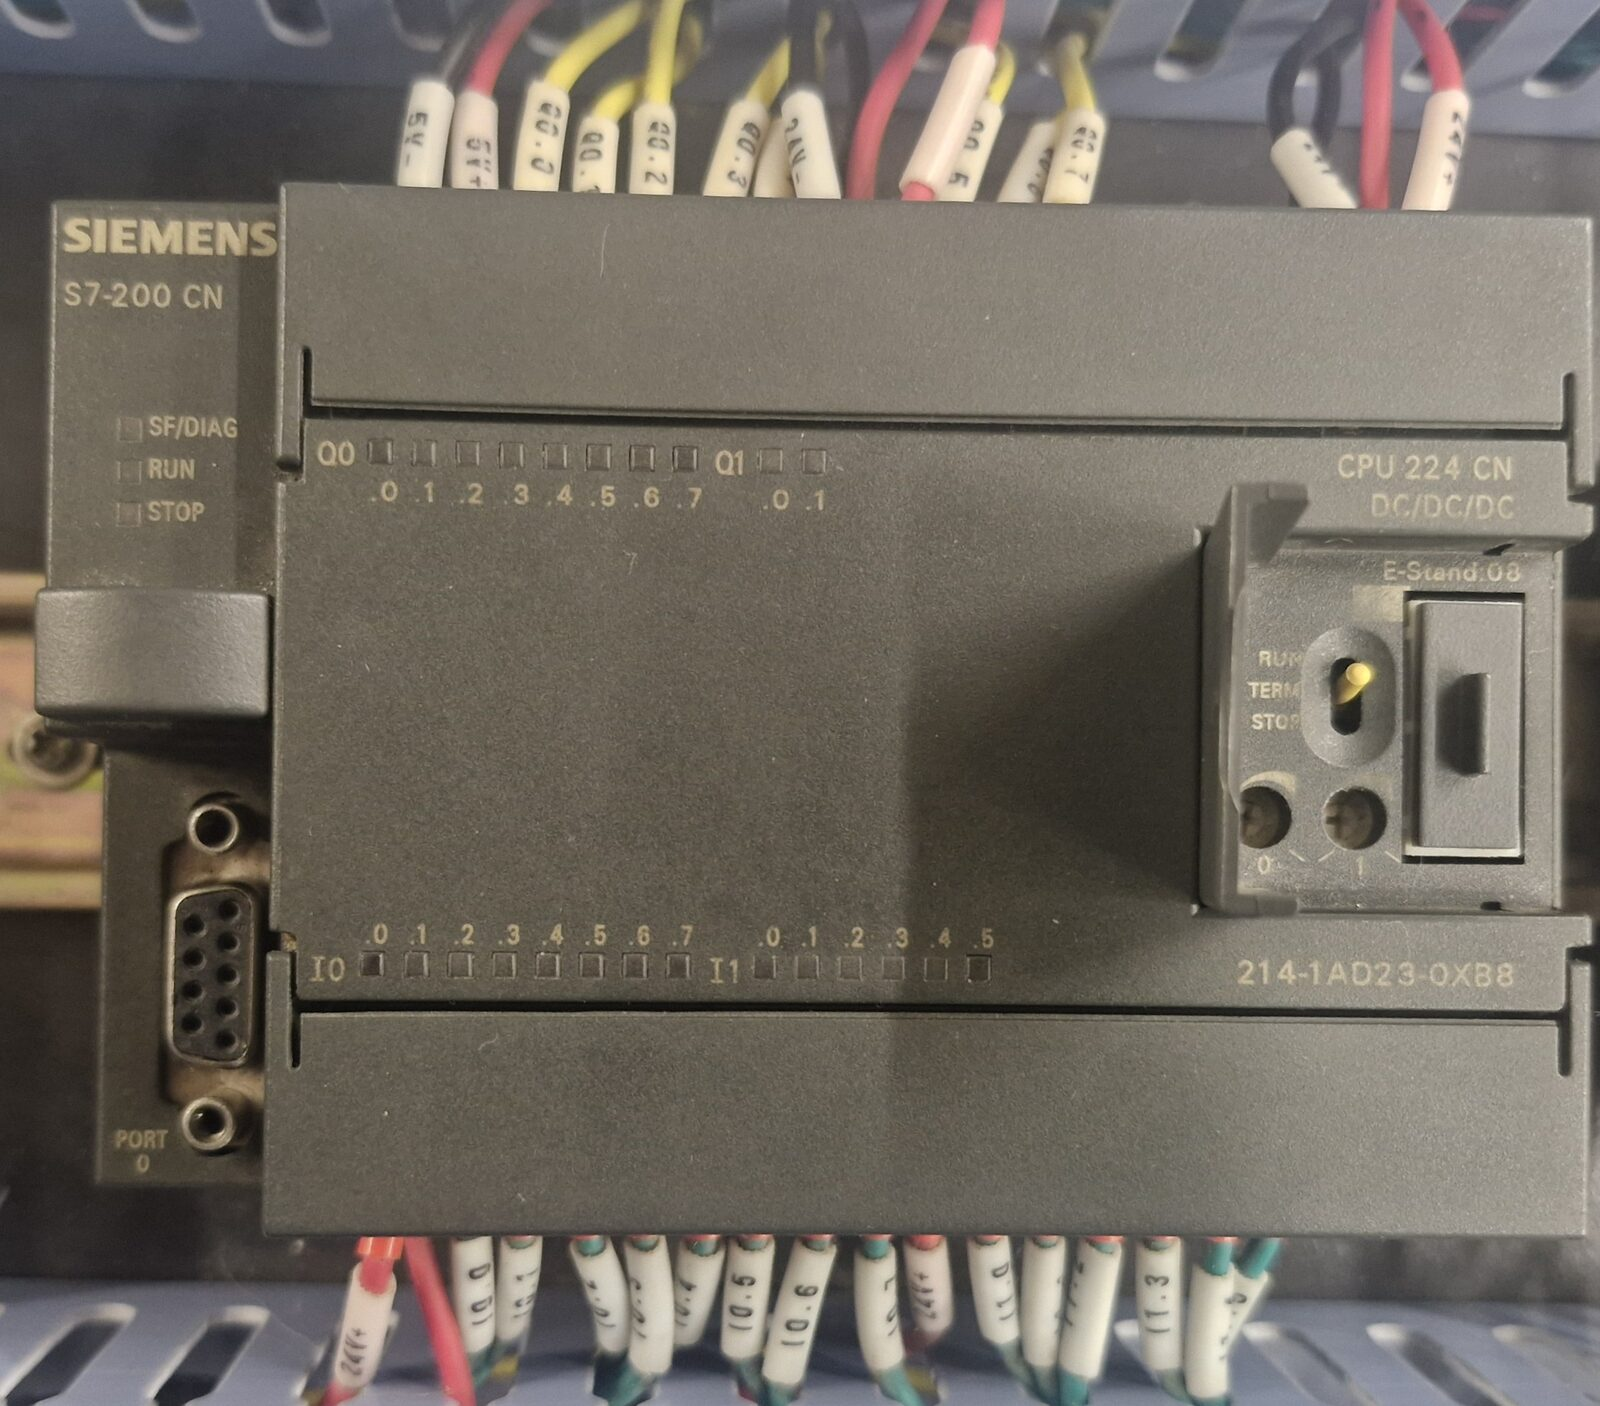
\includegraphics[width=\linewidth, height=3.6cm, keepaspectratio]{plc_s7-200_cpu224.jpg}\\{\small (a) PLC S7-200 CPU 224}\end{minipage}\hfill
\begin{minipage}[t]{0.32\linewidth}\centering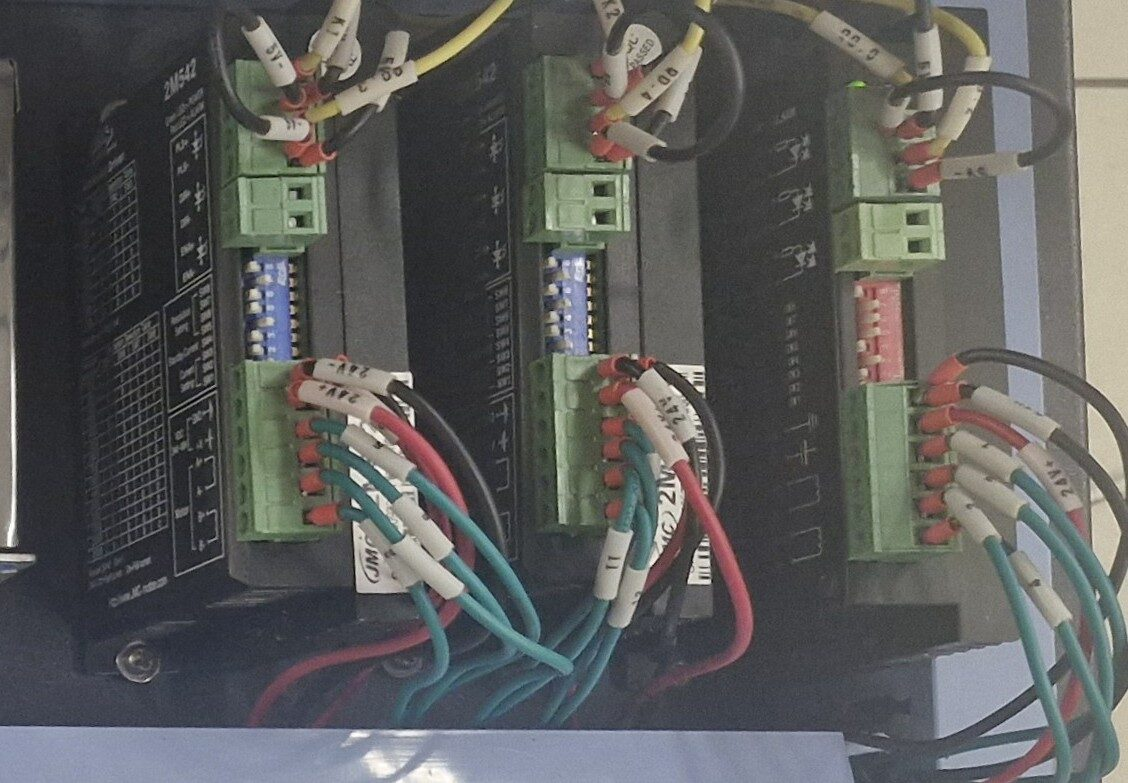
\includegraphics[width=\linewidth, height=3.6cm, keepaspectratio]{drivers_2m542_2m530.jpg}\\{\small (b) drivers 2M542 y 2M530}\end{minipage}\hfill
\begin{minipage}[t]{0.32\linewidth}\centering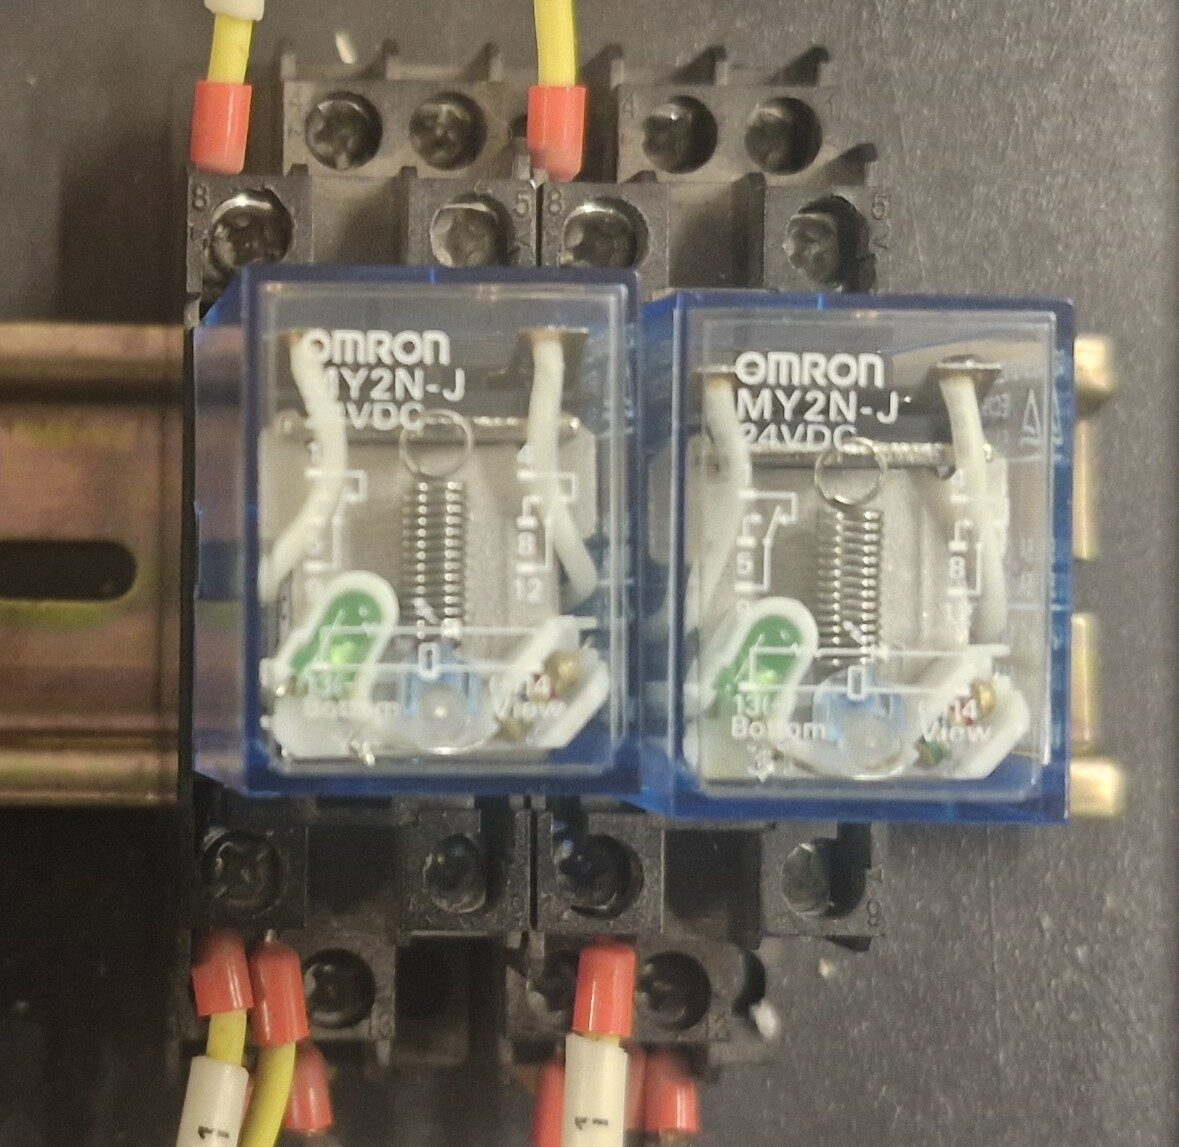
\includegraphics[width=\linewidth, height=3.6cm, keepaspectratio]{reles_omron_my2nj.jpg}\\{\small (c) relés Omron MY2N-J}\end{minipage}\\[6pt]
\begin{minipage}[t]{0.32\linewidth}\centering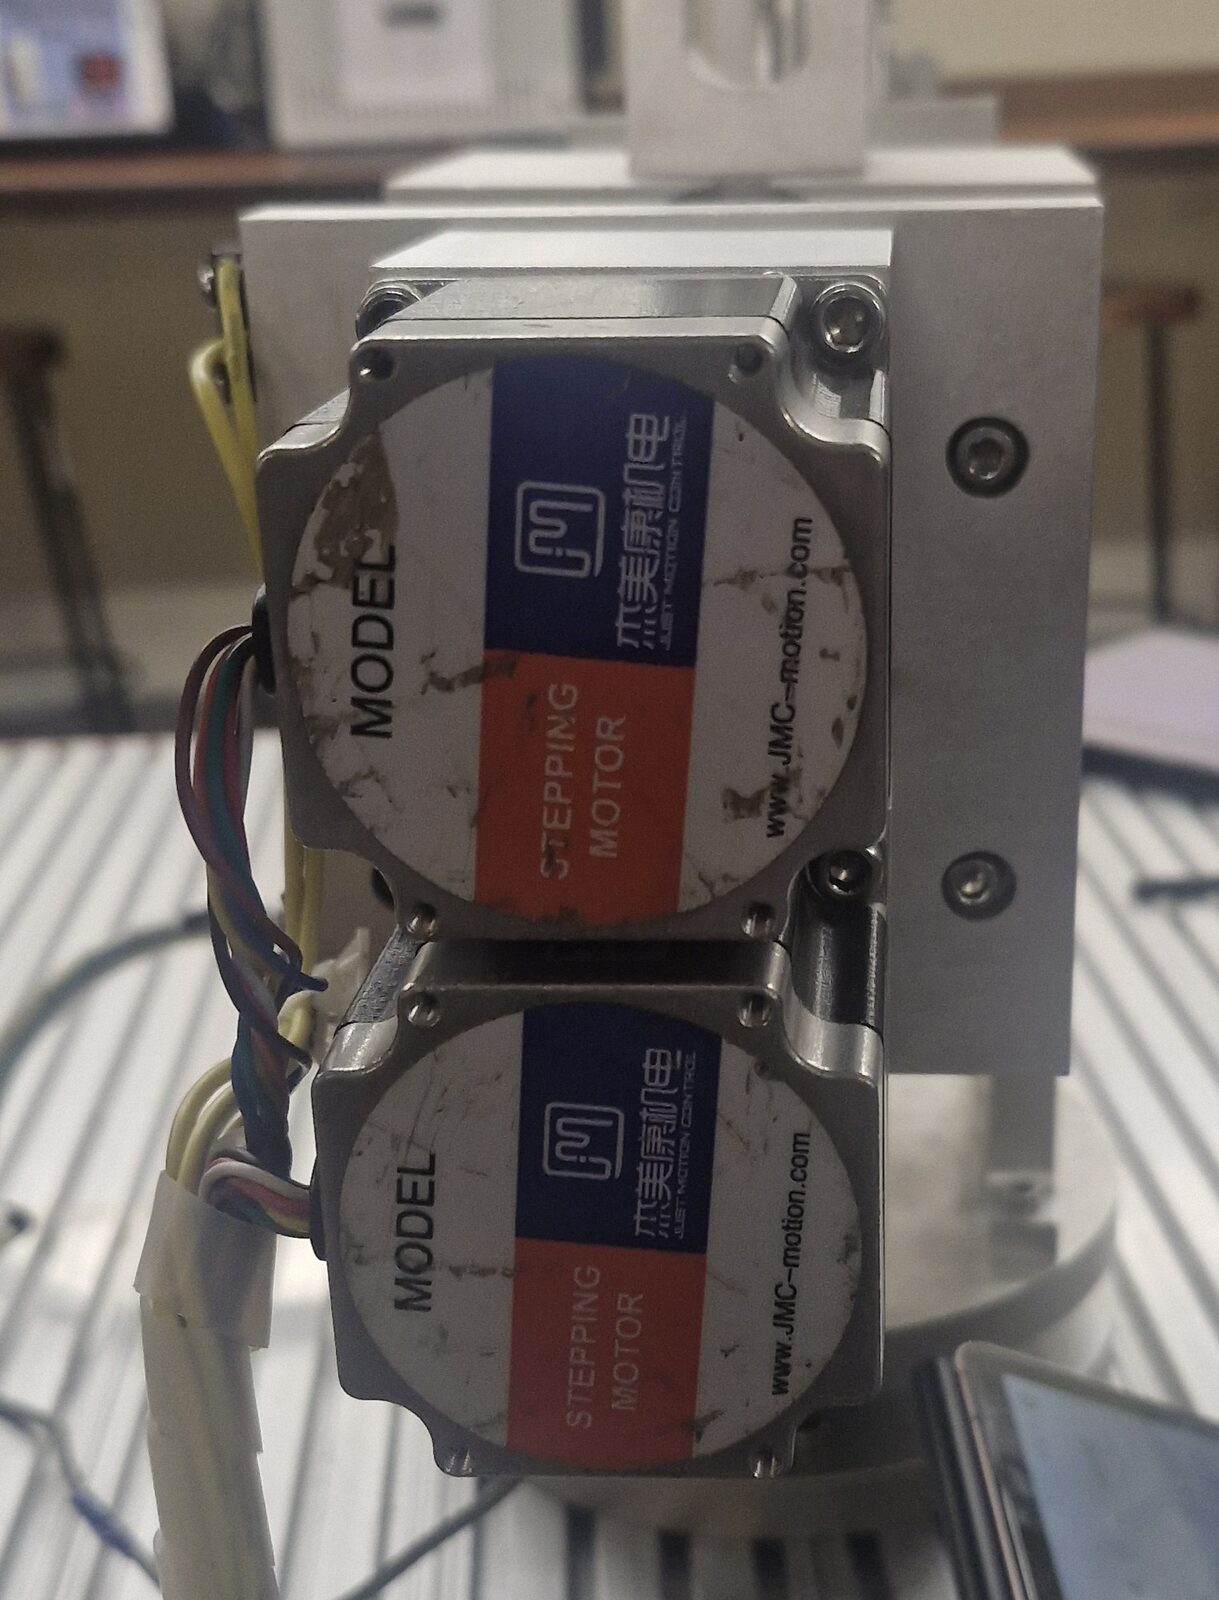
\includegraphics[width=\linewidth, height=3.6cm, keepaspectratio]{motores_nema23_ejes_xy.jpg}\\{\small (d) motores NEMA 23 (X, Y)}\end{minipage}\hfill
\begin{minipage}[t]{0.32\linewidth}\centering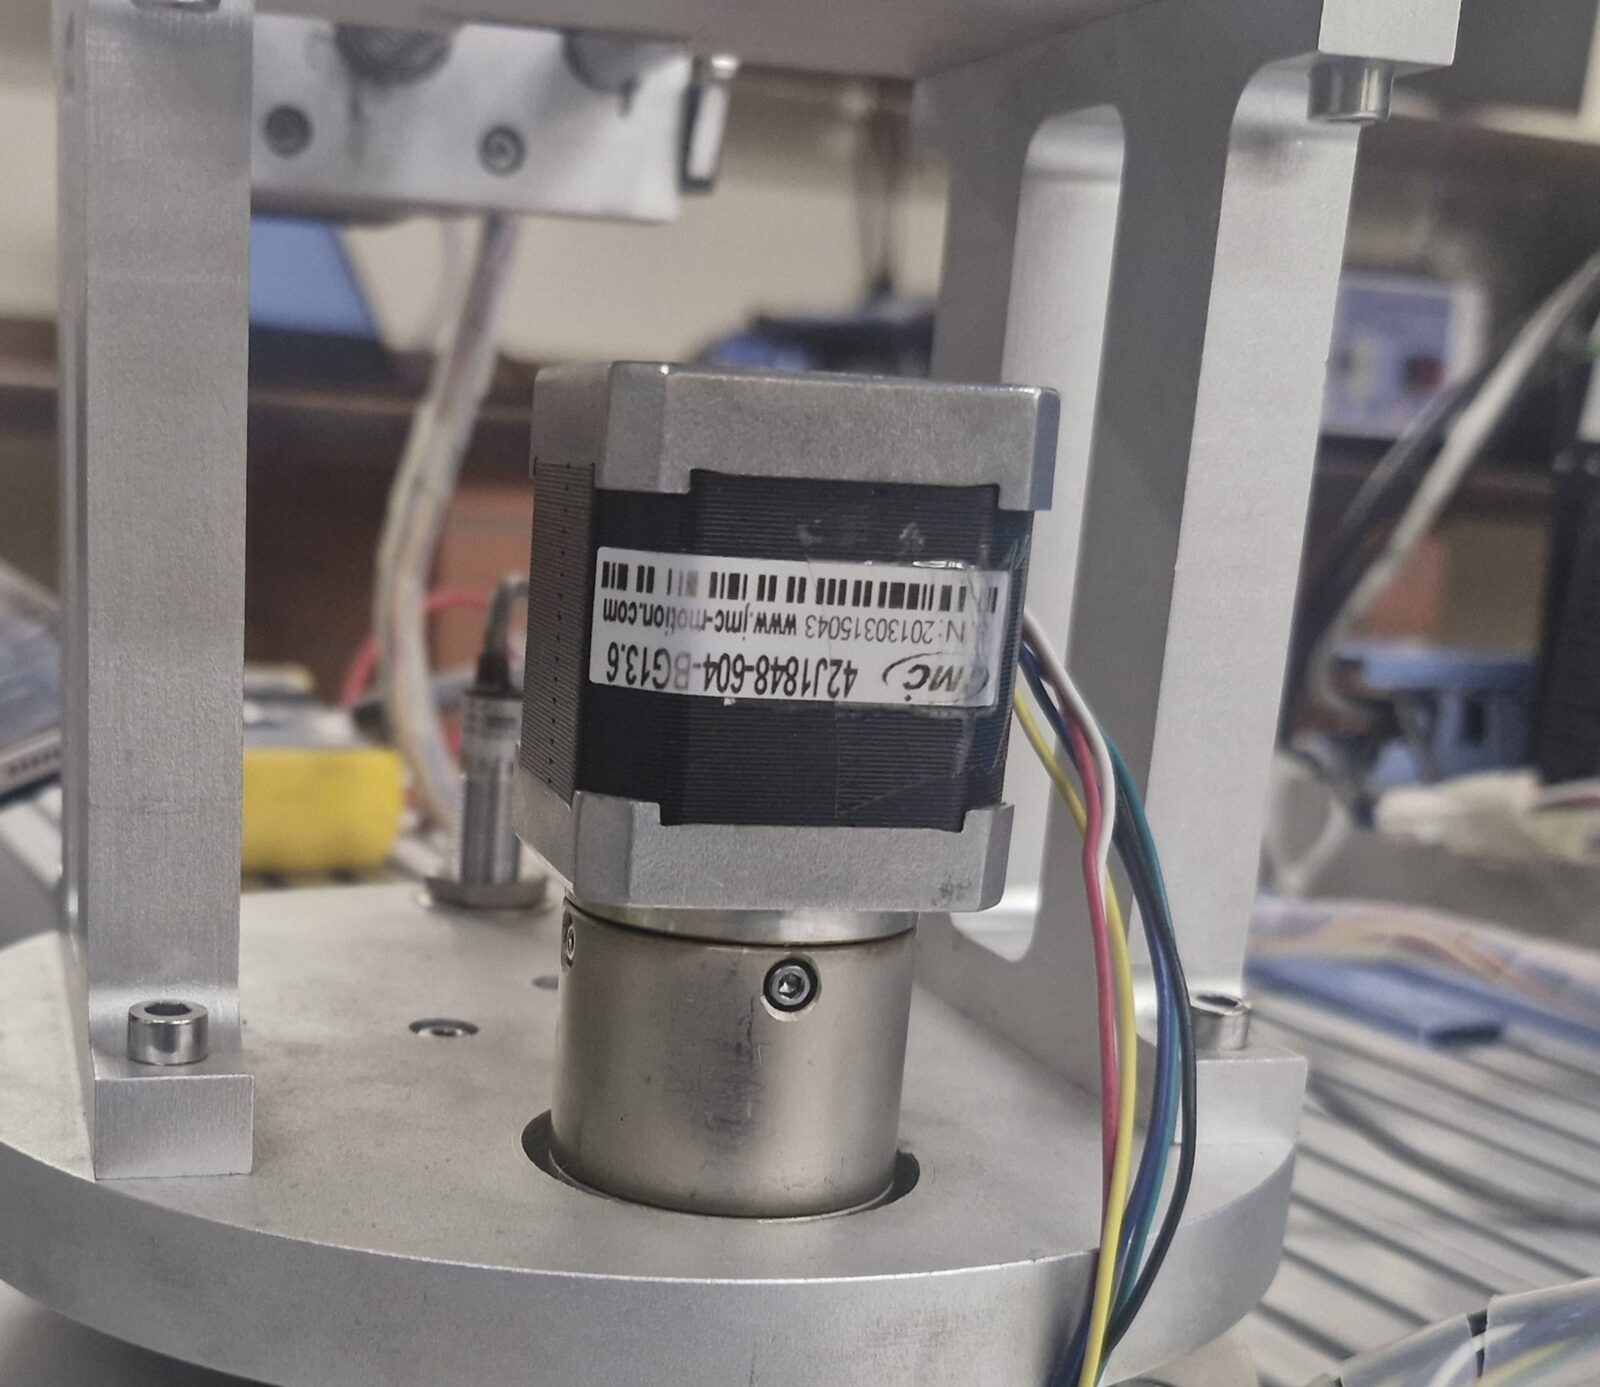
\includegraphics[width=\linewidth, height=3.6cm, keepaspectratio]{motor_nema17_eje_z.jpg}\\{\small (e) motor NEMA 17 (base)}\end{minipage}\hfill
\begin{minipage}[t]{0.32\linewidth}\centering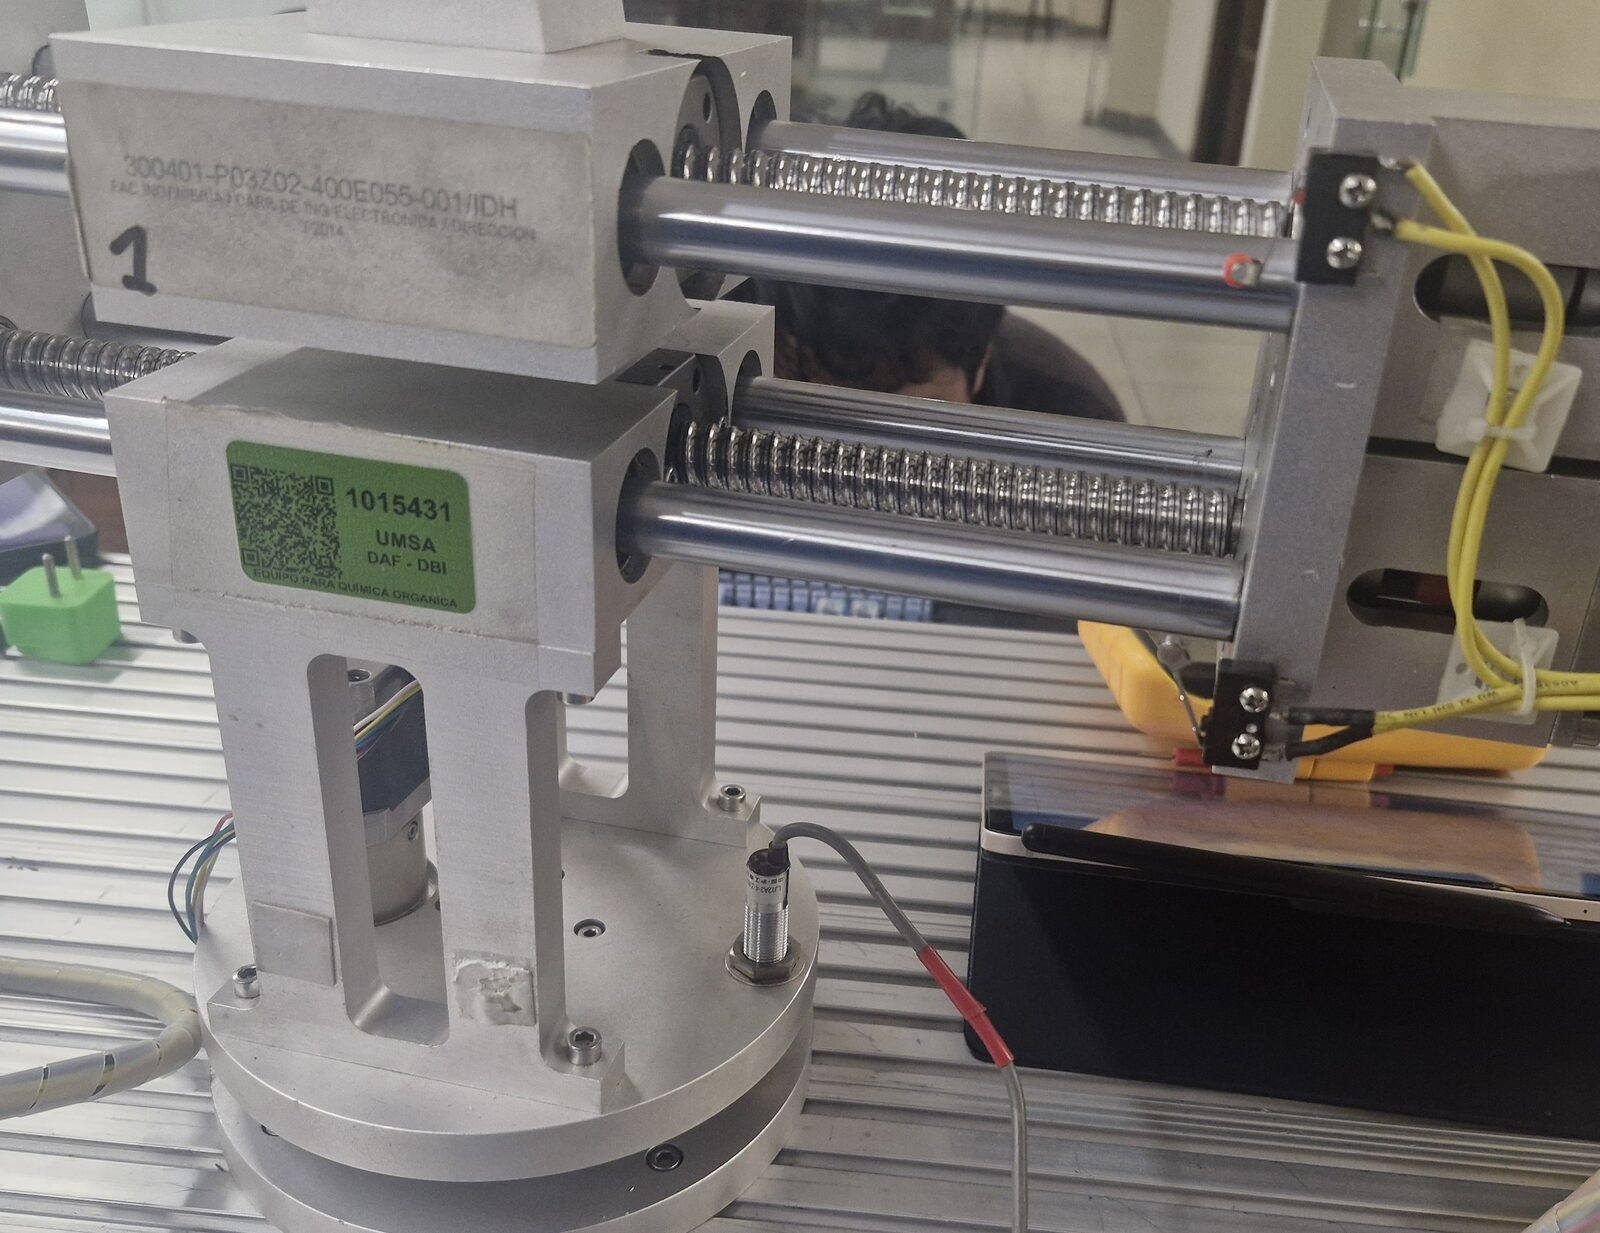
\includegraphics[width=\linewidth, height=3.6cm, keepaspectratio]{eje_z_sensor_inductivo.jpg}\\{\small (f) sensor inductivo de la base}\end{minipage}\\[6pt]
\begin{minipage}[t]{0.32\linewidth}\centering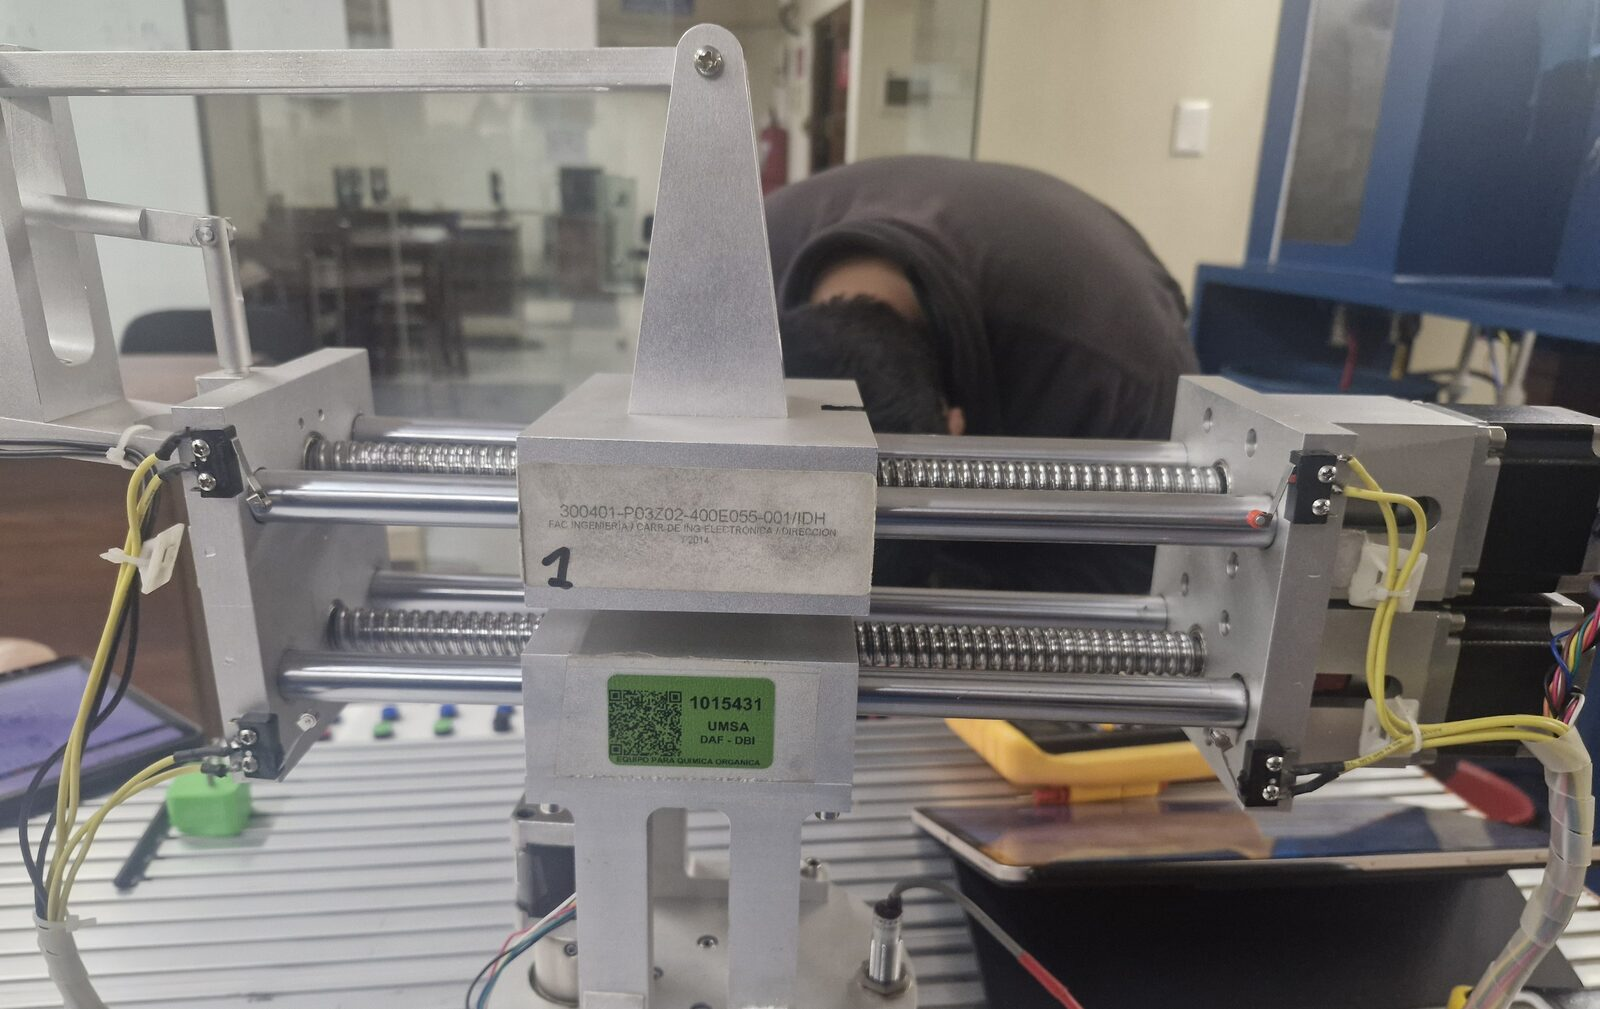
\includegraphics[width=\linewidth, height=3.6cm, keepaspectratio]{final_de_carrera_rieles_xy.jpg}\\{\small (g) finales de carrera X e Y}\end{minipage}\hfill
\begin{minipage}[t]{0.32\linewidth}\centering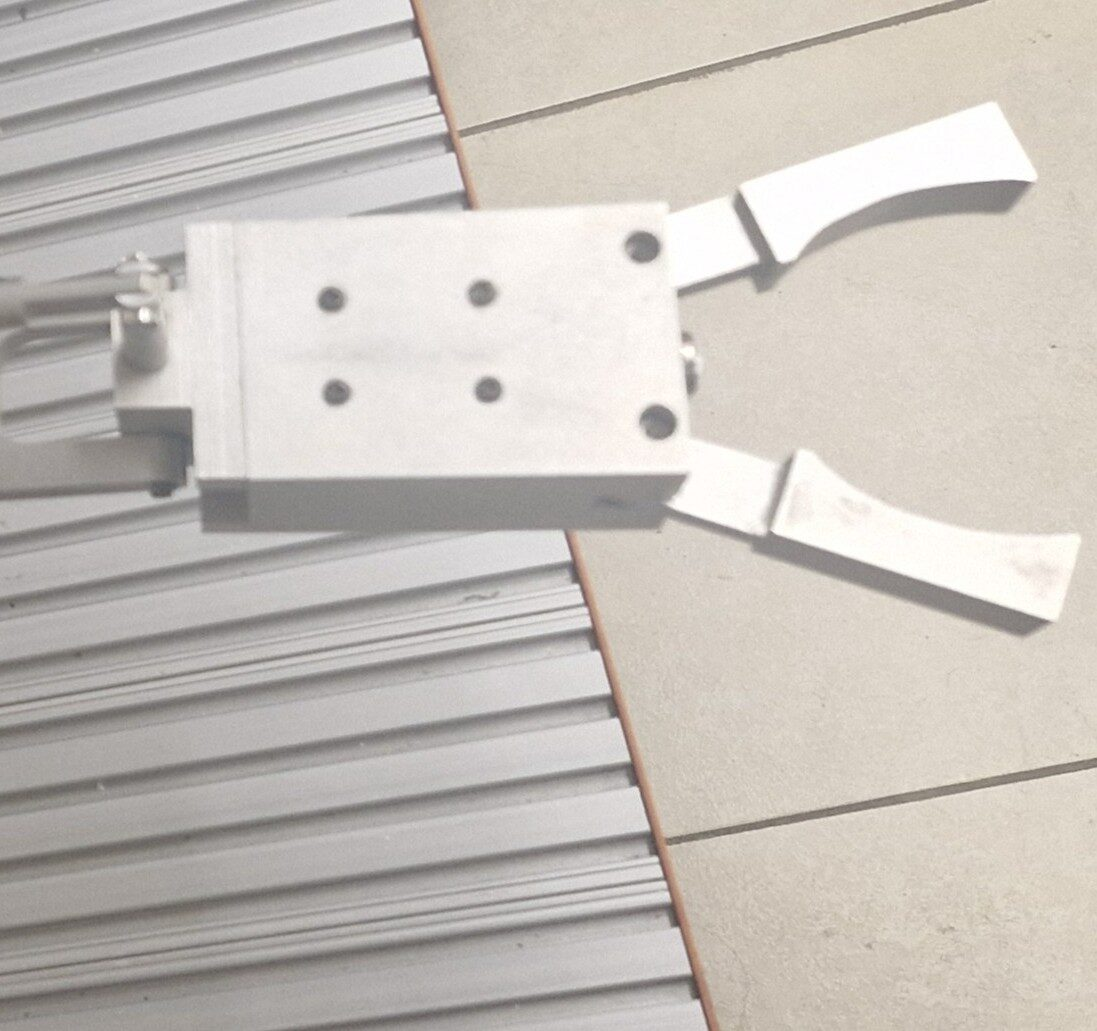
\includegraphics[width=\linewidth, height=3.6cm, keepaspectratio]{garra_solenoide.jpg}\\{\small (h) garra}\end{minipage}\hfill
\begin{minipage}[t]{0.32\linewidth}\centering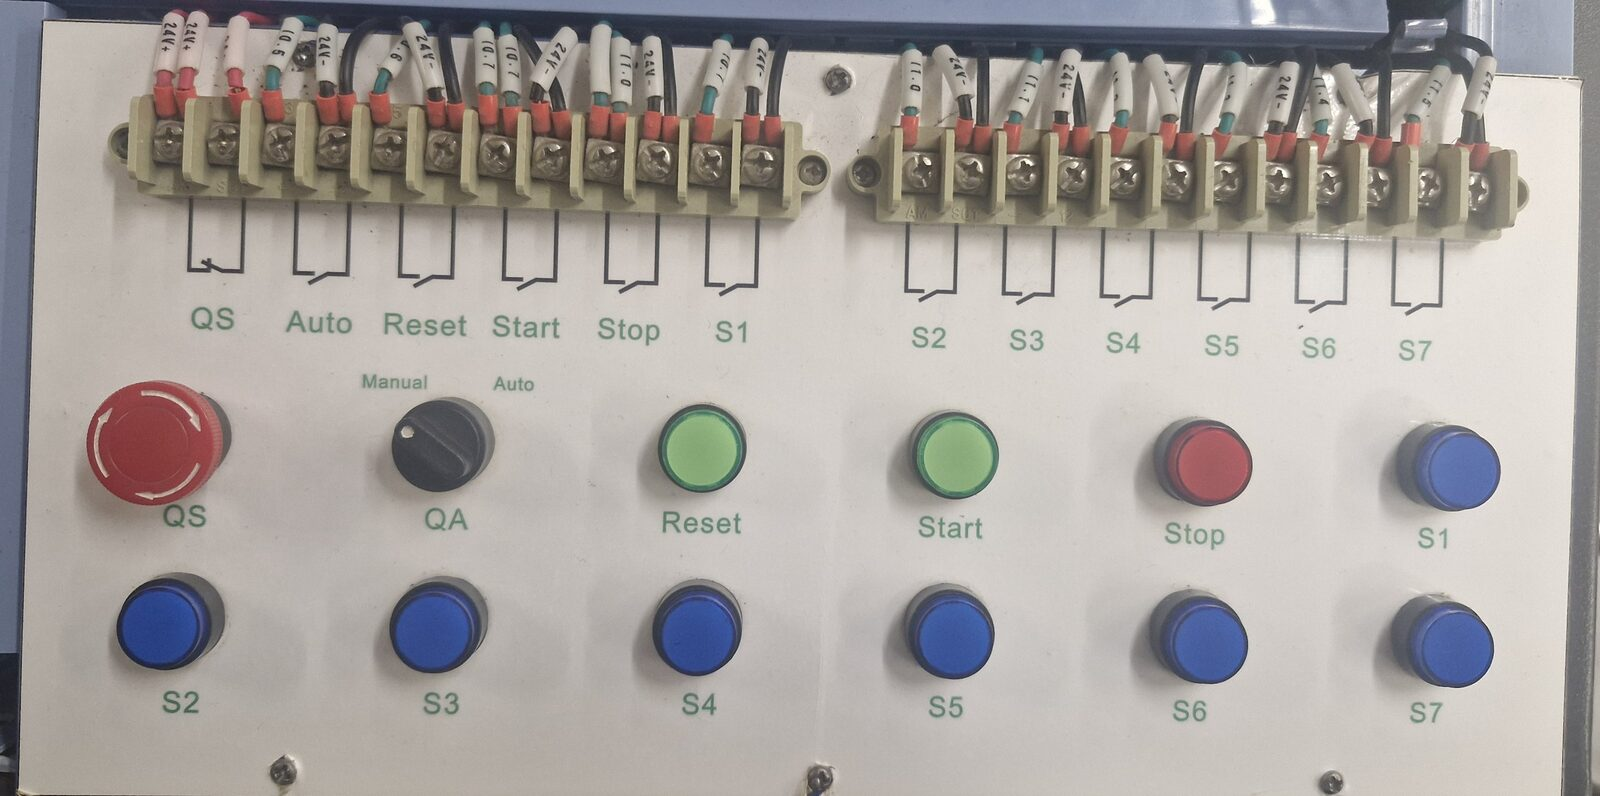
\includegraphics[width=\linewidth, height=3.6cm, keepaspectratio]{botonera.jpg}\\{\small (i) botonera}\end{minipage}
\caption{Componentes de la planta (fotos de \texttt{global/fotos-planta/}).}
\end{figure}

\section{Diagrama de bloques}
\begin{figure}[H]
\centering
\begin{tikzpicture}[node distance=7mm and 10mm]
\node[cajan, text width=3.1cm, minimum height=26mm] (plc) {\textbf{PLC S7-200}\\CPU 224 CN\\14 entradas\\10 salidas\\2 salidas de pulsos};
\node[caja, text width=2.6cm, above left=4mm and 14mm of plc] (panel) {panel:\\selector, paro,\\garra/inicio,\\6 pulsadores};
\node[caja, text width=2.6cm, below left=4mm and 14mm of plc] (sens) {finales de carrera X e Y\\sensor inductivo\\de la base};
\node[caja, text width=2.4cm, right=16mm of plc, yshift=16mm] (dz) {driver base\\2M530};
\node[caja, text width=2.4cm, right=16mm of plc, yshift=-4mm] (k) {relés K1 / K2\\reparten Q0.1};
\node[caja, text width=2.4cm, right=10mm of k, yshift=6mm] (dx) {driver X\\2M542};
\node[caja, text width=2.4cm, right=10mm of k, yshift=-8mm] (dy) {driver Y\\2M542};
\node[caja, text width=2.4cm, below=10mm of k] (garra) {relé K3 + solenoide\\de la garra};
\node[cajab, text width=1.6cm, right=6mm of dz] (mz) {NEMA 17\\base};
\node[cajab, text width=1.6cm, right=6mm of dx] (mx) {NEMA 23\\X};
\node[cajab, text width=1.6cm, right=6mm of dy] (my) {NEMA 23\\Y};
\node[cajab, text width=2.4cm, below=10mm of plc] (pc) {PC\\(USB-PPI, puerto 0)};
\draw[flecha] (panel) -- node[above, etiq, sloped]{I0.5--I1.5} (plc);
\draw[flecha] (sens) -- node[below, etiq, sloped]{I0.0--I0.4} (plc);
\draw[flecha] (plc.east) ++(0,0.6) -- node[above, etiq]{Q0.0, Q0.2} (dz.west);
\draw[flecha] (plc.east) ++(0,-0.4) -- node[above, etiq]{Q0.1} (k.west);
\draw[flecha] (k) -- node[above, etiq]{K1} (dx.west);
\draw[flecha] (k) -- node[below, etiq]{K2} (dy.west);
\draw[flecha] (plc.south east) -- node[above, etiq, sloped]{Q0.7} (garra.west);
\draw[flecha] (dz) -- (mz); \draw[flecha] (dx) -- (mx); \draw[flecha] (dy) -- (my);
\draw[dflecha] (plc) -- node[left, etiq]{PPI} (pc);
\node[etiq, above=1mm of dx] {DIR Q0.3};
\node[etiq, below=1mm of dy] {DIR Q0.4};
\end{tikzpicture}
\caption{Diagrama de bloques de la planta.}
\end{figure}

\section{Mapa de entradas y salidas verificado}
Cada sensor se accionó a mano mientras un monitor por PPI registraba los cambios (26/10/2026). Esto corrigió el mapa del informe 1 (sección \ref{sec:kaizen}).

\begin{center}\small
\begin{tabularx}{\linewidth}{>{\ttfamily}p{1.1cm} >{\raggedright}X >{\ttfamily}p{1.1cm} >{\raggedright\arraybackslash}X}
\toprule
\textbf{\rmfamily Entrada} & \textbf{Función} & \textbf{\rmfamily Salida} & \textbf{Función}\\
\midrule
I0.0 & sensor inductivo de la base ($\theta = 0$) & Q0.0 & pulsos de la base (PTO0)\\
I0.1 & final X atrás (origen) & Q0.1 & pulsos de X e Y (PTO1), compartidos\\
I0.2 & final X adelante & Q0.2 & DIR base (1 = hacia el inductivo)\\
I0.3 & final Y abajo (origen) & Q0.3 & DIR X (0 = adelante)\\
I0.4 & final Y arriba & Q0.4 & DIR Y (0 = arriba)\\
I0.5 & selector: 0 manual, 1 automático/remoto & Q0.5 & relé K1: Q0.1 al driver X\\
I0.6 & paro & Q0.6 & relé K2: Q0.1 al driver Y\\
I0.7 & garra / inicio & Q0.7 & relé K3: solenoide (1 = cerrada)\\
I1.0 / I1.1 & jog base + / $-$ & & \\
I1.2 / I1.3 & jog X adelante / atrás & & \\
I1.4 / I1.5 & jog Y arriba / abajo & & \\
\bottomrule
\end{tabularx}
\end{center}
La correspondencia entre los rótulos de la botonera (S1--S7, Start, Stop) y las entradas I0.6--I1.5 no se registró pulsador por pulsador (SUPUESTO: Stop = I0.6, Start = I0.7).

\section{Variables del proceso (PV, MV, DV)}
El brazo no tiene sensores de posición continua (encoders): la posición de cada eje se \emph{infiere} contando pulsos. Clasificación corregida respecto del informe 1:

\begin{center}\small
\begin{longtable}{>{\raggedright}p{1.3cm} >{\raggedright}p{4.2cm} >{\raggedright\arraybackslash}p{9.4cm}}
\toprule
\textbf{Tipo} & \textbf{Variable} & \textbf{Señal física y rango}\\
\midrule
\endhead
MV & tren de pulsos de la base ($N_\theta$, $f_\theta$) & Q0.0 (PTO0), 0--20~kHz; se usa 2,5--4~kHz\\
MV & tren de pulsos de X e Y ($N_{XY}$, $f_{XY}$) & Q0.1 (PTO1), uno solo para los dos carros\\
MV & selección de carro & Q0.5 (K1, carro X), Q0.6 (K2, carro Y)\\
MV & dirección de cada eje & Q0.2 (base), Q0.3 (X), Q0.4 (Y)\\
MV & garra & Q0.7, 24~V al relé K3\\
PV & posición de la base $\theta$ & sin sensor continuo; $\theta = n_\theta / 190{,}3$ [°]\\
PV & posición de los carros $s_X$, $s_Y$ & sin sensor continuo; $s = n / 200$ [mm], 0--170~mm\\
PV & posición de la garra $(X, Y, Z)$ & calculada con la cinemática directa (capítulo \ref{cap:cinematica})\\
PV discreta & referencias de posición & I0.0 (inductivo), I0.1--I0.4 (finales): solo dicen si se alcanzó un punto\\
DV & fricción en guías y husillos & no medible eléctricamente\\
DV & carga en la garra & peso de la pieza: cambia el par que necesita el carro Y\\
DV & pérdida de pasos & arranques sin rampa o sobrecarga: la posición contada deja de ser la real\\
DV & holguras y deformaciones & error de posición de la garra no detectable\\
\bottomrule
\end{longtable}
\end{center}

\section{Lazo abierto con supervisión discreta}
\begin{figure}[H]
\centering
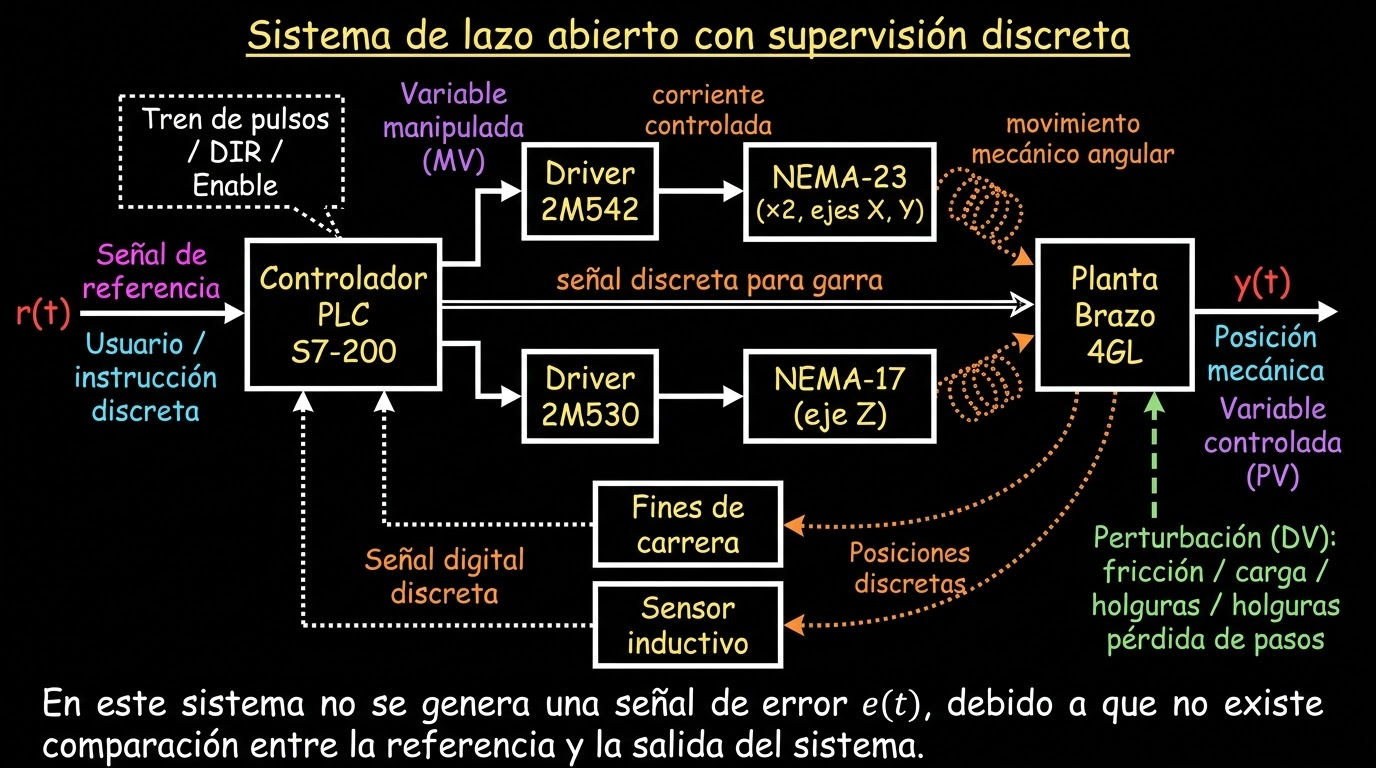
\includegraphics[width=0.8\linewidth]{diagrama_bloques_fenomenologico.png}
\caption{Diagrama de bloques fenomenológico del equipo (\texttt{diagramas/}): no hay realimentación continua de posición.}
\end{figure}
El PLC estima la posición como
\[
q_{est} = q_0 + N_p\,\Delta q ,
\]
donde $q_0$ es la posición de referencia (fijada por el homing), $N_p$ los pulsos enviados y $\Delta q$ el avance por pulso (0,005~mm en los carros). Si el motor pierde pasos, $q_{real} \neq q_{est}$ y el PLC no lo sabe: la acción de control actúa sobre la planta ($u \to y$) pero la salida no vuelve al controlador ($y \not\to u$). Es la \emph{ruptura de causalidad} del informe 1. Los finales de carrera solo corrigen la estimación en puntos aislados. El programa del gemelo aprovecha esto: cada vez que se pisa un final, fija la posición exacta (capítulo \ref{cap:gemeloplc}).

\section{Tags ISA-5.1 propuestos}
Para que los planos, el programa y la base de datos usen los mismos nombres (pedido de las guías 2 y 3), se propone esta identificación. La letra Z de ISA-5.1 designa \emph{posición}; S = interruptor; L/H = bajo/alto; Y = función de cálculo o relé; H = manual; I = indicación; X = sin clasificar.

\begin{center}\small
\begin{longtable}{>{\ttfamily}p{1.9cm} >{\ttfamily}p{1.2cm} >{\raggedright\arraybackslash}p{11cm}}
\toprule
\textbf{\rmfamily Tag} & \textbf{\rmfamily Señal} & \textbf{Descripción}\\
\midrule
\endhead
\multicolumn{3}{@{}l}{\textbf{Lazo 100: general}}\\
HS-100 & I0.5 & selector manual / automático\\
HS-100P & I0.6 & pulsador de paro\\
ZY-100 & Q0.1 & tren de pulsos compartido X/Y (PTO1)\\
\multicolumn{3}{@{}l}{\textbf{Lazo 101: base ($\theta$)}}\\
ZS-101 & I0.0 & interruptor de posición inductivo ($\theta = 0$)\\
HS-101A / B & I1.0 / I1.1 & jog base + / $-$\\
ZY-101 & Q0.0 & tren de pulsos de la base (PTO0)\\
ZY-101D & Q0.2 & dirección de la base\\
ZI-101 & VD1124 & posición de la base (pulsos contados)\\
\multicolumn{3}{@{}l}{\textbf{Lazo 102: carro X}}\\
ZSL-102 / ZSH-102 & I0.1 / I0.2 & final de carrera bajo (atrás) / alto (adelante)\\
HS-102A / B & I1.2 / I1.3 & jog X adelante / atrás\\
ZY-102D & Q0.3 & dirección X\\
ZY-102K & Q0.5 & relé K1\\
ZI-102 & VD1128 & posición X\\
\multicolumn{3}{@{}l}{\textbf{Lazo 103: carro Y}}\\
ZSL-103 / ZSH-103 & I0.3 / I0.4 & final de carrera bajo (abajo) / alto (arriba)\\
HS-103A / B & I1.4 / I1.5 & jog Y arriba / abajo\\
ZY-103D & Q0.4 & dirección Y\\
ZY-103K & Q0.6 & relé K2\\
ZI-103 & VD1132 & posición Y\\
\multicolumn{3}{@{}l}{\textbf{Lazo 104: garra}}\\
HS-104 & I0.7 & garra / inicio\\
XY-104 & Q0.7 & relé K3 del solenoide\\
\bottomrule
\end{longtable}
\end{center}
Los mismos tags están en la base de datos (tablas \codigo{punto\_io} y \codigo{variable}, capítulo \ref{cap:datos}).

\section{Discrepancias Kaizen: versión 2.0}\label{sec:kaizen}
El informe 1 registró discrepancias entre el plano histórico y la planta. La puesta en marcha del gemelo permitió verificarlas con el PLC en marcha y agregar otras:

\begin{center}\small
\begin{longtable}{>{\raggedright}p{0.4cm} >{\raggedright}p{4.4cm} >{\raggedright}p{4.6cm} >{\raggedright\arraybackslash}p{5.6cm}}
\toprule
\textbf{N°} & \textbf{Elemento} & \textbf{Antes} & \textbf{Verificado (oct. 2026)}\\
\midrule
\endhead
1 & finales de carrera & I0.0--I0.3 (informe 1, con desfase de 1 bit) & \textbf{I0.1--I0.4}; I0.0 es el inductivo de la base\\
2 & tren de pulsos de X e Y & Q0.5 (X) y Q0.6 (Y) & \textbf{Q0.1 compartido}; Q0.5 y Q0.6 son los relés K1 y K2 que lo reparten\\
3 & final de homing del carro Y & I0.4 (tabla anterior del proyecto) & \textbf{I0.3} (Y abajo)\\
4 & sentido de X & no documentado & Q0.3 = 0 adelante (se separa de I0.1)\\
5 & dirección PPI del PLC & 7 (proyecto de Miguel) & \textbf{6} a 19,2~kbit/s con el programa original; \textbf{2} a 9,6~kbit/s tras cargar \codigo{brazo\_gemelo} con su bloque de sistema\\
6 & reducción de la base & 5:1 (SUPUESTO del modelo) & \textbf{190,3 pulsos/°} medidos: unos 68,5 vueltas del motor por vuelta de la base (con 1000 pulsos/vuelta, SUPUESTO)\\
7 & driver de la base & mismo modelo que X/Y & 2M530 (otra tabla de corriente): revisar su configuración (capítulo \ref{cap:drivers})\\
8 & pines DIR+ de X e Y & sin conexión en el plano & conectados (informe 1); el plano debe corregirse\\
9 & garra & trazo incorrecto en el plano & salida Q0.7 $\rightarrow$ relé K3 $\rightarrow$ solenoide\\
\bottomrule
\end{longtable}
\end{center}
\pendiente{Pasar estas correcciones al plano eléctrico y al P\&ID en AutoCAD Electrical (versión 2.0 oficial, guía 2). Los archivos actuales están en \codigo{semestres/2026\_II/planos/}.}
